\chapter{Geodesics} \label{s:geo}

\minitoc

\section{Introduction}

Geodesics play a key role in general relativity, since they represent
the worldlines of test particles and photons
(cf. Sec.~\ref{s:fra:worldlines}). Moreover, in black hole theory,
null geodesics play a prominent role, as the generators of event horizons
(cf. Sec.~\ref{s:glo:properties_H}). We review here the definition and
main properties of geodesics on a generic pseudo-Riemannian manifold,
i.e. a manifold equipped with a metric of generic signature, as introduced in
Sec.~\ref{s:bas:pRiemManif}.
In particular, the results apply to pure Riemannian manifolds (positive
definite metric), as well as to Lorentzian manifolds, i.e.
spacetimes.
Contrary to Appendix~\ref{s:bas}, proofs of most statements will be provided,
since they are quite illustrative.

%%%%%%%%%%%%%%%%%%%%%%%%%%%%%%%%%%%%%%%%%%%%%%%%%%%%%%%%%%%%%%%%%%%%%%%%%%%%%%%

\section{Definition and first properties}

\subsection{Geodesics and affine parametrizations} \label{s:geo:def}

On a Riemannian manifold, i.e. when the metric tensor is positive definite
(cf. Sec.~\ref{s:bas:signature}), a geodesic is the curve of minimal length between
two points (at least for close enough points). It is also a curve which is
``as straight as possible'', in the sense that its tangent vectors are transported parallelly
to themselves along it. A typical example is a geodesic in the Euclidean space: this is
nothing but a straight line, for which tangent vectors
keep obviously a fixed direction. In a \emph{pseudo}-Riemannian manifold, such as the
spacetimes of general relativity, one uses
this last property to define geodesics.

Let us first recall the basic definitions given in Sec.~\ref{s:bas:vectors}:
a \defin{curve}\index{curve}\footnote{As already noticed (cf. Remark~\ref{r:bas:curve_def} p.~\pageref{r:bas:curve_def}), in the mathematical literature, it is common to define
a curve as the parametrization itself, and not as its image.}
is the image $\Li=P(I)$
of a map (called a \defin{parametrization} of the curve)
$P:\ I\rightarrow \M$, $\lambda\mapsto P(\lambda)$,
where $I$ is an interval of $\R$ and the variable $\lambda$ is called a
\defin{parameter} of the curve.
Moreover, we exclude the case where $\Li$ is reduced to a single point
of $\M$, i.e. where $P$ is a constant function.
We are now in position to define a geodesic as a ``straight'' curve:

\begin{greybox}
A smooth curve $\Li$ of a pseudo-Riemannian manifold $(\M,\w{g})$ is
called a \defin{geodesic} iff it admits a parametrization $P$ whose associated
tangent vector field $\w{v}$ is transported parallelly to itself along
$\Li$:
\be \label{e:geo:geod_eq_v}
    \encadre{\wnab_{\!\w{v}} \w{v} = 0},
\ee
where $\wnab$ is the Levi-Civita connection of the metric $\w{g}$.
The parametrization $P$ is then called an
\defin{affine parametrization}\index{affine!parametrization}\index{parametrization!affine --}
and the corresponding parameter $\lambda$ is called an
\defin{affine paramater}\index{affine!parameter}\index{parameter!affine --} of the
geodesic $\Li$. Note that the relation between $\w{v}$ and $\lambda$ is
\be \label{e:geo:v_dxdlambda}
    \w{v} = \frac{\D\w{x}}{\D\lambda} ,
\ee
where $\D\w{x}$ is the infinitesimal displacement along $\Li$ corresponding
to the change $\D\lambda$ in the parameter $\lambda$
(cf. Eq.~(\ref{e:bas:dell_v_dlamb})).
\end{greybox}

The qualifier \emph{affine} in the above definition stems from the following
property:
\begin{greybox}
Any two affine parametrizations of a geodesic $\Li$ are necessarily
related by an affine transformation:
\be \label{e:geo:affine_transf}
    \lambda' = a \lambda + b,
\ee
where $a$ and $b$ are two real constants such that $a\not = 0$.
\end{greybox}
\begin{proof}
Let $P: I \to  \Li\subset\M$, $\lambda\mapsto P(\lambda)$ and
$P': I'\to \Li$,
$\lambda'\mapsto P'(\lambda')$ be two
parametrizations of $\Li$. They are necessarily related by a
diffeomorphism $I\to I'$, $\lambda \mapsto \lambda'(\lambda)$. It follows
from Eq.~(\ref{e:geo:v_dxdlambda}) that the tangent vector fields $\w{v}$ and $\w{v'}$
associated with these two parametrizations are related by
\be  \label{e:geo:change_tangent_vector}
    \w{v} = \frac{\D\lambda'}{\D\lambda} \, \w{v'} .
\ee
Using the rules 2 and 3 governing the connection $\wnab$ (cf. Sec.~\ref{s:bas:affine_connect}),
we get then
\be \label{e:geo:acc_v_acc_vp}
    \wnab_{\!\w{v}}\w{v} = \frac{\D^2\lambda'}{\D\lambda^2} \, \w{v'}
    + \left( \frac{\D\lambda'}{\D\lambda} \right)^2 \wnab_{\!\w{v'}}\w{v'} .
\ee
If both parametrizations are affine, then $\wnab_{\!\w{v}}\w{v} = 0$ and
$\wnab_{\!\w{v'}}\w{v'} = 0$, so that the above identity reduces to
${\D^2\lambda'}/{\D\lambda^2} = 0$, which implies
the affine law (\ref{e:geo:affine_transf}).
\end{proof}

\begin{remark}
Because of (\ref{e:geo:geod_eq_v}), a geodesic is also called
an \defin{autoparallel curve}\index{autoparallel}. It is also sometimes called
a \defin{zero-acceleration curve}\index{zero-acceleration}, the
vector $\wnab_{\!\w{v}}\w{v}$ being considered as the
``acceleration''\index{acceleration! of a curve} of (the parametrization $P$ of) the
curve $\Li$; this is of course by extension of the concept of
4-acceleration $\w{a} := \wnab_{\!\w{u}}\w{u}$ of a timelike worldline
with 4-velocity $\w{u}$, the latter being nothing but the tangent vector associated with
the parametrization of the worldline by its proper time (cf. Sec.~\ref{s:fra:massive_part}).
\end{remark}

An important property of geodesics is
\begin{greybox}
Let $\Li$ be a geodesic of $(\M,\w{g})$ and $\w{v}$ a tangent vector field
associated with an affine parametrization of $\Li$. Then the
scalar square of $\w{v}$ with respect to the metric $\w{g}$
is constant along $\Li$:
\be \label{e:geo:vv_const}
    \w{g}(\w{v},\w{v}) = \mathrm{const}.
\ee
\end{greybox}
\begin{proof}
The variation of $\w{g}(\w{v},\w{v})$ along $\Li$ is given
by
\bea
 \frac{\D}{\D\lambda}  \left( \w{g}(\w{v},\w{v}) \right) & = & \w{v} \left( \w{g}(\w{v},\w{v}) \right)
    = \wnab_{\!\w{v}} \left( \w{g}(\w{v},\w{v}) \right) = v^\mu \nabla_\mu (g_{\rho\sigma} v^\rho v^\sigma) \nonumber \\
            & = & v^\mu \underbrace{\nabla_\mu g_{\rho\sigma}}_{0} v^\rho v^\sigma
                + g_{\rho\sigma} \underbrace{v^\mu \nabla_\mu v^\rho}_{0} v^\sigma
                + g_{\rho\sigma} v^\rho \underbrace{v^\mu \nabla_\mu v^\sigma}_{0} = 0 , \nonumber
\eea
where we have used the fact that $\wnab$ is the Levi-Civita connection of $\w{g}$ [Eq.~(\ref{e:bas:nabla_g_zero})] and $\w{v}$ obeys the geodesic equation (\ref{e:geo:geod_eq_v}).
\end{proof}
The constancy of $\w{g}(\w{v},\w{v})$ has an
interesting corollary: the tangent vector $\w{v}$ cannot change its type
along $\Li$. Hence:
\begin{greybox}
In a pseudo-Riemannian manifold $(\M,\w{g})$, a geodesic $\Li$ belongs necessarily
to one of the following three categories:
\begin{itemize}
\item \defin{timelike geodesic}\index{timelike!geodesic}\index{geodesic!timelike --}:
tangent vectors are timelike at all points of $\Li$;
\item \defin{null geodesic}\index{null!geodesic}\index{geodesic!null --}:
tangent vectors are null at all points of $\Li$;
\item \defin{spacelike geodesic}\index{spacelike!geodesic}\index{geodesic!spacelike --}:
tangent vectors are spacelike at all points of $\Li$.
\end{itemize}
\end{greybox}
This is in sharp contrast with generic curves, which, for instance, can be timelike on some portions
and null or spacelike on other parts.

In the timelike case, or the spacelike one,
the tangent vector field $\w{v}$ can be rescaled by the constant $\sqrt{|\w{g}(\w{v},\w{v})|}$ to get
a unit tangent vector field, i.e. a tangent vector field $\w{u}$ which obeys
$\w{g}(\w{u},\w{u}) = -1$ (timelike geodesic) or $\w{g}(\w{u},\w{u}) = 1$
(spacelike geodesic). Moreover, in doing so, the affine character of the
parametrization is preserved. Indeed, the rescaling amounts to choosing the constant $a$
in the affine law~(\ref{e:geo:affine_transf}) such that $a = \sqrt{|\w{g}(\w{v},\w{v})|}$.
Thus, we have
\begin{greybox}
A timelike or spacelike geodesic of a Lorentzian manifold has an affine parametrization,
the tangent vector of which is a unit vector (i.e. of scalar square $\pm 1$ with respect to
$\w{g}$). Moreover this parametrization is unique up to some choice of origin
(choice of $b$ in (\ref{e:geo:affine_transf})) and of
orientation ($a=\pm 1$ in (\ref{e:geo:affine_transf})).
\end{greybox}
We shall see in Sec.~\ref{s:geo:gener_param} that for a timelike geodesic,
the affine parameter with unit tangent vector is nothing but the
\emph{proper time}\index{proper!time}\index{time!proper --}, while for a spacelike
geodesic, it is the \emph{arc length}\index{arc length}.

\subsection{Generic parametrizations of geodesics} \label{s:geo:gener_param}

Geodesics can be characterized by any of their tangent vectors, i.e.
tangent vectors not necessarily associated with an affine parametrization, as follows:
\begin{greybox}
A curve $\Li$ is a geodesic
iff the tangent vector field $\w{v}$ associated with any parametrization
of $\Li$ obeys
\be \label{e:geo:v_pregeodesic}
    \wnab_{\!\w{v}}\w{v} = \kappa\,  \w{v},
\ee
where $\kappa$ is a scalar field along $\Li$.
\end{greybox}
\begin{proof}
Let $P: I\to \Li$, $\lambda\mapsto P(\lambda)$ be the parametrization of $\Li$
corresponding to the tangent vector field $\w{v}$: $\w{v} = \D\w{x}/\D\lambda$.
If $\Li$ is a geodesic, then there exists a parametrization
$\lambda'\mapsto P'(\lambda')$ whose tangent vector, $\w{v'}$ say, obeys
$\wnab_{\!\w{v'}}\w{v'} = 0$. Since the accelerations of any two parametrizations of $\Li$
are related by Eq.~(\ref{e:geo:acc_v_acc_vp}), we deduce that $\w{v}$ obeys
(\ref{e:geo:v_pregeodesic}) with
\[
    \kappa = \left( \frac{\D\lambda'}{\D\lambda} \right)^{-1}
        \frac{\D^2\lambda'}{\D\lambda^2} .
\]
Conversely, if $\w{v}$ obeys (\ref{e:geo:v_pregeodesic}) with $\kappa=\kappa(\lambda)$,
then Eq.~(\ref{e:geo:acc_v_acc_vp}) implies that $\wnab_{\!\w{v'}}\w{v'} = 0$,
i.e. that $\Li$ is a geodesic, provided that the change of
parametrization $\lambda' = \lambda'(\lambda)$ fulfils
\[
    \kappa(\lambda) \frac{\D\lambda'}{\D\lambda} -  \frac{\D^2\lambda'}{\D\lambda^2} = 0 .
\]
This differential equation has the following solution:
\[
    \lambda' = a \int_{\lambda_1}^\lambda \left[ \exp \left(
    \int_{\lambda_0}^{\tilde{\lambda}} \kappa(\tilde{\tilde{\lambda}})
    \D\tilde{\tilde{\lambda}}\right) \D\tilde\lambda
    \right] + b,
\]
where $a$, $b$, $\lambda_0$ and $\lambda_1$ are constants, with $a\not = 0$ and $\lambda_0,\lambda_1\in I$.
\end{proof}
The above property motivates the following definitions:
\begin{greybox}
A vector field $\w{v}$ obeying (\ref{e:geo:v_pregeodesic}) is called
a \defin{pregeodesic vector field}\index{pregeodesic!vector field}.
The scalar field $\kappa$ is then called the \defin{non-affinity coefficient}\index{non-affinity coefficient} of $\w{v}$.
If $\kappa=0$, $\w{v}$ is naturally called a \defin{geodesic vector field}\index{geodesic!vector field}.
\end{greybox}
Note that the property established above is equivalent to stating that the
field lines of a pregeodesic vector field are geodesics.

An easy consequence of Eq.~(\ref{e:geo:v_pregeodesic}) is the following
evolution law for the scalar square of the tangent vector:
\begin{greybox}
Along a geodesic $\Li$, the scalar square $\w{g}(\w{v},\w{v})$
of the tangent vector $\w{v}$ associated with any parametrization of $\Li$
evolves according to
\be \label{e:geo:evol_vv_kappa}
    \wnab_{\!\w{v}} \left[ \w{g}(\w{v},\w{v}) \right] = 2 \kappa \, \w{g}(\w{v},\w{v}),
\ee
where $\kappa$ is the non-affinity coefficient of $\w{v}$.
\end{greybox}
\begin{proof}
One has, using $\wnab\w{g}=0$ [Eq.~(\ref{e:bas:nabla_g_zero})] and Eq.~(\ref{e:geo:v_pregeodesic}),
\[
    v^\mu \nabla_\mu (g_{\rho\sigma} v^\rho v^\sigma)  = v^\mu \underbrace{\nabla_\mu g_{\rho\sigma}}_{0} v^\rho v^\sigma
                + g_{\rho\sigma} \underbrace{v^\mu \nabla_\mu v^\rho}_{\kappa v^\rho} v^\sigma
                + g_{\rho\sigma} v^\rho \underbrace{v^\mu \nabla_\mu v^\sigma}_{\kappa v^\sigma}
             = 2 \kappa  g_{\rho\sigma} v^\rho v^\sigma  ,
\]
hence the law (\ref{e:geo:evol_vv_kappa}).
\end{proof}
We recover of course (\ref{e:geo:vv_const}) in the special case $\kappa = 0$
($\w{v}$ geodesic vector).
\begin{remark}
If $\lambda$ is the parameter associated with $\w{v}$, i.e. $\w{v} = \D\w{x}/\D\lambda$,
we may introduce the scalar function $V(\lambda) := \w{g}(\w{v},\w{v})$ and
rewrite (\ref{e:geo:evol_vv_kappa}) as a first-order ordinary differential equation
for it [cf. Eq.~(\ref{e:bas:def_vector})]:
\be
    \frac{\D V}{\D\lambda} = 2 \kappa(\lambda) V(\lambda) .
\ee
\end{remark}
A consequence of (\ref{e:geo:evol_vv_kappa}) is
\begin{greybox}
On a Lorentzian manifold, the parametrization of a timelike geodesic
by the proper time\index{time!proper --} ($\lambda = \tau$) is an affine parametrization.
Similarly, on a Lorentzian or Riemannian manifold, the parametrization of a
spacelike geodesic
by the arc length\index{arc length} ($\lambda = s$) is an affine parametrization.
\end{greybox}
\begin{proof}
The tangent vector associated with the proper time $\tau$ along a timelike geodesic
is nothing but the 4-velocity $\w{u}$ (cf. Sec.~\ref{s:fra:massive_part}), which
is of constant scalar square: $\w{g}(\w{u},\w{u}) = -1$, so that Eq.~(\ref{e:geo:evol_vv_kappa})
reduces to $0 = -2 \kappa$, hence $\kappa=0$, which implies that we are dealing
with an affine parametrization. Similarly, the tangent vector associated with the
arc length $s$ along a spacelike geodesic has a scalar square everywhere equal
to 1, leading to the same conclusion.
\end{proof}

%%%%%%%%%%%%%%%%%%%%%%%%%%%%%%%%%%%%%%%%%%%%%%%%%%%%%%%%%%%%%%%%%%%%%%%%%%%%%%%

\section{Existence and uniqueness of geodesics}

\subsection{The geodesic equation}

\begin{greybox}
Let $\Li$ be a curve in a pseudo-Riemannian
manifold $(\M,\w{g})$ of dimension $n$, such that
$\Li$ is contained in the domain of a coordinate chart $(x^\alpha)_{0\leq\alpha\leq n-1}$.
Then any parametrization of $\Li$, $P: I \to  \Li$, $\lambda\mapsto P(\lambda)$,
can be described by $n$ functions $X^\alpha: I\to \R$
according to Eq.~(\ref{e:bas:curve_param_equation}): $x^\alpha(P(\lambda)) = X^\alpha(\lambda)$.
The curve $\Li$ is a geodesic iff there exists a parametrization of $\Li$
for which the functions $X^\alpha$ fulfils the following
system of $n$ second-order differential equations, called the
\defin{geodesic equation}\index{geodesic!equation}\index{equation!geodesic --}:
\be \label{e:geo:eq_geod}
    \encadre{ \frac{\D^2 X^\alpha}{\D\lambda^2} + \Gamma^\alpha_{\ \, \mu \nu}
    \frac{\D X^\mu}{\D\lambda} \frac{\D X^\nu}{\D\lambda} = 0 },  \qquad 0 \leq \alpha \leq n-1,
\ee
where the $\Gamma^\alpha_{\ \, \mu \nu}$'s are the Christoffel symbols\index{Christoffel symbols} of the metric $\w{g}$
with respect to the coordinates $(x^\alpha)$, as given by Eq.~(\ref{e:bas:Christoffel}).
\end{greybox}
\begin{proof}
Notice first that the components with respect
to the chart $(x^\alpha)$ of the tangent
vector field $\w{v}$ associated with the parameter $\lambda$ are [cf. Eq.~(\ref{e:bas:va_dXadlamb})]
\be \label{e:geo:va_dXadlamb}
    v^\alpha = \frac{\D X^\alpha}{\D\lambda} .
\ee
On the other side, the components of $\wnab_{\!\w{v}}\w{v}$ are
\[
    v^\mu \nabla_\mu v^\alpha = v^\mu \der{v^\alpha}{x^\mu} + \Gamma^\alpha_{\ \, \mu \nu} v^\mu v^\nu
    = \w{v}(v^\alpha) + \Gamma^\alpha_{\ \, \mu \nu} v^\mu v^\nu
    = \frac{\D v^\alpha}{\D \lambda} + \Gamma^\alpha_{\ \, \mu \nu} v^\mu v^\nu ,
\]
where we have used
successively Eqs.~(\ref{e:bas:der_cov_coord}), (\ref{e:bas:v_va_wpar_a}) and
(\ref{e:bas:def_vector}). The above relation, along with (\ref{e:geo:va_dXadlamb}),
shows that the left-hand side of
Eq.~(\ref{e:geo:eq_geod}) is nothing but the component $\alpha$ of
$\wnab_{\!\w{v}}\w{v}$. The conclusion follows from the very definition
of a geodesic given in Sec.~\ref{s:geo:def}.
\end{proof}

Note that if a solution of the geodesic equation (\ref{e:geo:eq_geod}) is found, the parameter
$\lambda$ is necessarily an affine parameter.
For a generic parameter,
the differential equation becomes (\ref{e:geo:eq_geod}) with the right-hand side
replaced by $\kappa \D X^\alpha /\D\lambda$, which is the coordinate
expression of the right-hand side $\kappa \w{v}$ in
Eq.~(\ref{e:geo:v_pregeodesic}). Hence, we have
\begin{greybox}
A curve $\Li$ in the domain of a chart $(x^\alpha)$ is a geodesic
iff some (actually all) coordinate expression $x^\alpha = X^\alpha(\lambda)$
of $\Li$ fulfils the following
system of $n$ second-order differential equations, usually called the
\defin{pregeodesic equation}\index{pregeodesic!equation}\index{equation!pregeodesic --},
\be \label{e:geo:pregeod_eq_comp}
    \encadre{ \frac{\D^2 X^\alpha}{\D\lambda^2} + \Gamma^\alpha_{\ \, \mu \nu}
    \frac{\D X^\mu}{\D\lambda} \frac{\D X^\nu}{\D\lambda} =
    \kappa(\lambda) \frac{\D X^\alpha}{\D\lambda}   },  \qquad 0 \leq \alpha \leq n-1 .
\ee
for some real-valued function $\kappa(\lambda)$.
\end{greybox}

\subsection{Existence and uniqueness} \label{s:geo:existence_uniqueness}

We may use the geodesic equation to prove the following existence and uniqueness
theorem:
\begin{greybox}
Given a point $p$ in a pseudo-Riemannian manifold $(\M,\w{g})$ and a vector
$\w{V}$ in the tangent space to $\M$ at $p$, i.e. $\w{V} \in T_p\M$,
there exists a geodesic $\Li$ through $p$ such that
$\w{V}$ is the value at $p$ of the tangent vector of some affine parametrization
of $\Li$:
\be
    \w{V} = \left. \frac{\D\w{x}}{\D\lambda} \right|_p .
\ee
Moreover, this geodesic is unique, in the sense that any geodesic $\Li'$
sharing the same property coincides with $\Li$
in some open neighbourhood of $p$.
\end{greybox}
\begin{proof}
Let $(x^\alpha)$ be a coordinate chart of $\M$ around $p$. Let $(V^\alpha)$
be the components of $\w{V}$ in the basis of $T_p\M$ induced by
the coordinate frame $(\wpar_\alpha)$ associated with $(x^\alpha)$:
\[
    \w{V} = V^\alpha \left. \wpar_\alpha \right| _p .
\]
A geodesic through $p$ having $\w{V}$ as tangent vector at $p$ is then
obtained as a solution $(X^\alpha(\lambda))$ of the system (\ref{e:geo:eq_geod})
with the initial conditions [cf. Eq.~(\ref{e:geo:va_dXadlamb})]
\be \label{e:geo:init_cond}
    X^\alpha(0) = x^\alpha(p) \quad\mbox{and}\quad
    \frac{\D X^\alpha}{\D\lambda}(0) = V^\alpha .
\ee
The system (\ref{e:geo:eq_geod}) + (\ref{e:geo:init_cond}) constitutes a well-posed
Cauchy problem\index{Cauchy problem} and standard results about ordinary
differential equations, e.g. the Picard-Lindelöf (or Cauchy–Lipschitz) theorem,
guarantee the existence and uniqueness of the solution.
\end{proof}

A few definitions follow naturally:

\begin{greybox}
A geodesic $\Li$ is said to be \defin{inextendible}\index{inextendible geodesic}\index{geodesic!inextendible --}
or \defin{maximal}\index{maximal!geodesic}\index{geodesic!maximal --}
iff
there does not exist any geodesic $\Li'$ such that  $\Li\subset\Li'$ and
$\Li'\not=\Li$.
\end{greybox}

\begin{greybox}
A geodesic $\Li$ is \defin{complete}\index{complete!geodesic}\index{geodesic!complete --}
iff (i) it is inextendible and (ii) the interval spanned by any of its affine parameters is the whole real line:
$I=\R$. A geodesic that is not complete is called \defin{incomplete}\index{incomplete geodesic}\index{geodesic!incomplete --}.

The pseudo-Riemannian manifold $(\M,\w{g})$ is said to be
\defin{geodesically complete}\index{geodesically complete}\index{complete!geodesically -- spacetime}
iff every inextendible geodesic is complete.
\end{greybox}

\begin{remark}
A well-known theorem of differential geometry, namely the \defin{Hopf-Rinow theorem}\index{Hopf-Rinow theorem},
states that a connected \emph{Riemannian} manifold is geodesically complete iff it is \emph{complete}
as a \emph{metric space}\index{metric!space} for the distance function $d(p,q)$ defined as the infimum of
the length\footnote{The length of a curve is defined by Eq.~(\ref{e:geo:def_length}) below.} of all curves from $p$ to $q$
(see e.g. Ref.~\cite{Lee97}). However, there is no such theorem for \emph{Lorentzian}
manifolds, for the metric does not induce any distance function turning them into a metric space.
\end{remark}


The following proposition strengthens the existence and uniqueness
result obtained above:
\begin{greybox}
Given a point $p$ in a pseudo-Riemannian manifold $(\M,\w{g})$ and a
nonzero vector
$\w{V}$ in the tangent space to $\M$ at $p$, i.e. $\w{V} \in T_p\M$,
there exists a unique inextendible geodesic through $p$, which we shall denote
by $\Li_{\w{V}}$, such that
$\w{V}$ is the value at $p$ of the tangent vector of some affine parametrization
of $\Li_{\w{V}}$. We shall then denote by $P_{\w{V}}$ the unique
affine parametrization of $\Li_{\w{V}}$ such that
\be
    P_{\w{V}}(0) = p \quad\mbox{and}\quad \left.\w{v}\right| _p = \w{V} ,
\ee
where $\w{v}$ is the tangent vector field of
$P_{\w{V}}$.
\end{greybox}
We refer to O'Neill's textbook \cite{ONeil83}, p.~68 for the proof.

\goodbreak

\subsection{Exponential map}

One can make use of geodesics to map a tangent space to
the base manifold:

\begin{greybox}
Given a point $p$ in a pseudo-Riemannian manifold $(\M,\w{g})$,
let $\mathcal{E}_p$ be the subset of the tangent space $T_p\M$ defined
by $\w{V}\in \mathcal{E}_p$ iff either $\w{V}=0$ or
the affine parametrization $P_{\w{V}}$
of the geodesic $\Li_{\w{V}}$
has a domain large enough to include the interval $[0,1]$.
The \defin{exponential map at $p$}\index{exponential map} is then defined as
\be
    \begin{array}{cccl}
    \exp_p : & \mathcal{E}_p \subset T_p\M & \longrightarrow & \M \\
    & \w{V} & \longmapsto &
    \left\{ \begin{array}{ll}
        p &  \mbox{if}\ \w{V}=0 \\
        P_{\w{V}}(1) \in \Li_{\w{V}} & \mbox{if}\ \w{V}\not=0
        \end{array} \right.
    \end{array}
\ee
\end{greybox}
In other words, $\exp_p$ maps a nonzero vector $\w{V}$ in the tangent space to $\M$ at $p$
to the point of $\M$ of affine parameter $\lambda=1$
along the unique geodesic through $p$, the parameter $\lambda$ being such
that (i) $\lambda=0$ corresponds to $p$ and (ii) the associated tangent vector
$\D\w{x}/\D\lambda$ at $p$ is $\w{V}$.

Note that if $(\M,\w{g})$ is geodesically complete, $\mathcal{E}_p = T_p\M$
for every point $p\in\M$.

An immediate property of the exponential map is
\begin{greybox}
If $\w{V}\in \mathcal{E}_p\setminus\{0\}$, for any $t\in[0,1]$, $\exp_p(t\w{V})$ lies
on the same geodesic $\Li_{\w{V}}$ as $\exp_p(\w{V})$, at the parameter
$\lambda=t$ of the parametrization $P_{\w{V}}$:
\be \label{e:geo:exp_tV}
    \forall t\in[0,1],\quad \exp_p(t\w{V}) = P_{\w{V}}(t) .
\ee
\end{greybox}
\begin{proof}
For $t=0$, the property follows from the definition of $\exp_p$, since
$P_{\w{V}}(0) = p$.
If $t\not=0$, the nonzero vector $t\w{V}$ is collinear to $\w{V}$ and the uniqueness
property of geodesics (cf. Sec.~\ref{s:geo:existence_uniqueness})
implies that $\Li_{t\w{V}} = \Li_{\w{V}}$. By virtue
of the transformation law (\ref{e:geo:change_tangent_vector}), $t\w{V}$ is
the tangent vector to $\Li_{\w{V}}$ corresponding to the affine parameter
$\lambda' = t^{-1} \lambda$, where $\lambda$ is the affine parameter whose
tangent vector field obeys $\left.\w{v}\right| _p = \w{V}$. From the definition
of $\exp_p$, we have then $\exp_p(t\w{V}) = P_{t\w{V}}(\lambda'=1) = P_{\w{V}}(\lambda = t\times 1)$,
hence (\ref{e:geo:exp_tV}).
\end{proof}

The exponential map realizes a local identification of the manifold
with its tangent space at a given point:
\begin{greybox}
For any $p\in\M$, there exists a neighbourhood $U$ of $0$ in the tangent
space $T_p\M$ and a neighbourhood $\mathscr{U}$ of $p$ in the manifold $\M$
such that the exponential map $\exp_p$ is a diffeomorphism from
$U$ to $\mathscr{U}$.
\end{greybox}
\begin{proof}
It is clear from its definition that $\exp_p$ is a smooth map, at least
on some neighbourhood $U'$ of $0$ in $T_p\M$. We may then consider the
differential of $\exp_p$ at $0$, $\left.\D\exp_p\right| _0$.
By virtue of the inverse function theorem for manifolds (see e.g. Theorem~4.5 in
Ref.~\cite{Lee13}), it suffices to show that
$\left.\D\exp_p\right| _0$ is invertible to complete the proof.
By definition of the differential of a map (cf. Sec.~\ref{s:bas:embed})
and since $\exp_p: \mathcal{E}_p \subset T_p\M \to \M$
and $\exp_p(0) = p$, $\left.\D\exp_p\right| _0$ carries an
infinitesimal displacement vector of\footnote{Here the vector space $T_p\M$ is considered
as a $n$-dimensional smooth manifold, and $T_0(T_p\M)$ stands for its tangent space
at $0$ (the zero vector of $T_p\M$).} $T_0(T_p\M)$, $\w{\varepsilon}$ say, connecting $0$ to a nearby element of $T_p\M$, $\w{\varepsilon'}$ say,
to the infinitesimal vector $\w{E}\in T_p\M$ connecting
$p=\exp_p(0)$ to $q=\exp_p(\w{\varepsilon'})$:
\[
    \begin{array}{cccl}
    \left.\D\exp_p\right| _0: & T_0(T_p\M) & \longrightarrow & T_p\M \\
        & \w{\varepsilon} & \longmapsto & \w{E} = \vp{pq}.
    \end{array}
\]
Now, since $T_p\M$ is a vector space, we have the canonical identification
$T_0(T_p\M) \simeq T_p\M$, from which $\w{\varepsilon'} = \w{\varepsilon}$.
Without any loss of generality, we may write $\w{\varepsilon} = \varepsilon \w{V}$,
where $\varepsilon$ is infinitesimal small and $\w{V}\in T_p\M$. Then
$q = \exp_p(\varepsilon \w{V}) = P_{\w{V}}(\varepsilon)$, where the second
identity results from (\ref{e:geo:exp_tV}). We have thus
\[
    \left.\D\exp_p\right| _0(\varepsilon \w{V}) = \w{E} = \vp{pq} =
    \vp{P_{\w{V}}(0) P_{\w{V}}(\varepsilon)} .
\]
According to the definition of $P_{\w{V}}$, the infinitesimal vector
$\vp{P_{\w{V}}(0) P_{\w{V}}(\varepsilon)}$ along the geodesic $\Li_{\w{V}}$
is $\varepsilon \w{V}$, hence
\[
    \left.\D\exp_p\right| _0(\varepsilon \w{V}) = \varepsilon \w{V} .
\]
Since the differential $\left.\D\exp_p\right| _0$ is a linear map, we
get $\left.\D\exp_p\right| _0(\w{V}) = \w{V}$. The vector $\w{V}$ being arbitrary,
we conclude that $\left.\D\exp_p\right| _0$ is nothing but the identity map of
the vector space $T_p\M$:
\[
    \left.\D\exp_p\right| _0 = \operatorname{id}_{T_p\M} .
\]
In particular, $\left.\D\exp_p\right| _0$ is invertible.
\end{proof}

\subsection{Normal coordinates} \label{s:geo:normal_coord}

\begin{greybox}
Given $p\in\M$, a \defin{normal neighbourhood}\index{normal!neighbourhood}\index{neighbourhood!normal --}
of $p$ is a neighbourhood $\mathscr{U}$ of $p$ that is the image of a
starshaped neighbourhood of $0\in T_p\M$ under the local diffeomorphism
$\exp_p$ given by the above proposition.
By \defin{starshaped neighbourhood}\index{starshaped neighbourhood} of $0$, it
is meant a neighbourhood $U$ of $0$ such that $\w{V}\in U$
implies $t\w{V}\in U$ for any $t\in[0,1]$.
\end{greybox}

On a normal neighbourhood, one may define coordinates linked to geodesics
as follows.

\begin{greybox}
Let $\mathscr{U}$ be a normal neighbourhood of $p\in\M$ and $(\w{E}_\alpha)_{0\leq \alpha\leq n-1}$
be a basis of $T_p\M$. If $(\w{E}^\alpha)$ stands for the basis of $T_p^*\M$
dual to $(\w{E}_\alpha)$, the map
\be \label{e:geo:def_normal_coord}
     \begin{array}{cccl}
     \Phi: & \mathscr{U} & \longrightarrow & \R^n \\
        & q & \longmapsto & \left(\langle \w{E}^0, \exp_p^{-1}(q)\rangle, \ldots,
          \langle\w{E}^{n-1}, \exp_p^{-1}(q) \rangle \right)
     \end{array}
\ee
is a coordinate chart on $\mathscr{U}$, which is called
\defin{geodesic normal coordinates}\index{geodesic!normal coordinates}\index{coordinates!normal --},
often shorten as \defin{normal coordinates}\index{normal!coordinates}.
\end{greybox}
In other words, normal coordinates $(x^\alpha)$ on $\mathscr{U}$ are such
that the tangent vector $x^\mu(q) \w{E}_\mu\in T_p\M$ has precisely
$q$ as image by the exponential map:
\be
    \forall q \in \mathscr{U},\quad \exp_p(x^\mu(q) \w{E}_\mu) = q .
\ee
\begin{remark}
Some authors, e.g. \cite{ONeil83}, add the condition that the basis $(\w{E}_\alpha)$
is orthonormal (with respect to the metric $\w{g}$) in the definition of normal
coordinates. We follow here the more general definition of \cite{KobayN63,BishoG68,HawkiE73,Strau04}.
The name \defin{Riemann normal coordinates}\index{Riemann!normal coordinates}\index{normal!coordinates!Riemann --} is also commonly encountered in the literature,
either for normal coordinates as defined here (e.g. \cite{MisneTW73,Wald84})
or for those with the basis orthonormality requirement (e.g. \cite{PoissW14}).
\end{remark}

A characteristic feature of normal coordinates is that, in terms of them,
geodesics through $p$ look like straight lines through $0$ in
$\R^n$:
\begin{greybox}
In a normal coordinate system $(x^\alpha)$, the equation of the unique geodesic
$\Li_{\w{V}}$ through $p$ admitting $\w{V}\in T_p\M$ as tangent
vector at $p$ is (as long as $\Li_{\w{V}}$ remains in the normal
neighbourhood $\mathscr{U}$)
\be \label{e:geo:Xa_normal_coord}
    x^\alpha = X^\alpha(\lambda) = \lambda V^\alpha ,
\ee
where the $V^\alpha$'s are the components of $\w{V}$ with respect to the basis
$(\w{E}_\alpha)$ defining the normal coordinates: $\w{V} = V^\mu \w{E}_\mu$.
\end{greybox}
\begin{proof}
Let $\lambda$ be the affine parameter of $\Li_{\w{V}}$ corresponding
to the parametrization $P_{\w{V}}$. The coordinate equation of
$\Li_{\w{V}}$ is then $x^\alpha = X^\alpha(\lambda)$ with [cf. Eq.~(\ref{e:geo:def_normal_coord})]
\[
    X^\alpha(\lambda) = x^\alpha\left( P_{\w{V}}(\lambda) \right)
        = \langle \w{E}^\alpha, \exp_p^{-1} \left( P_{\w{V}}(\lambda) \right) \rangle .
\]
Now, according to Eq.~(\ref{e:geo:exp_tV}), $P_{\w{V}}(\lambda) = \exp_p (\lambda \w{V})$.
Hence
\[
    X^\alpha(\lambda) = \langle \w{E}^\alpha, \exp_p^{-1} \circ \exp_p (\lambda \w{V}) \rangle
     = \langle \w{E}^\alpha, \lambda \w{V} \rangle
        = \lambda \langle \w{E}^\alpha, \w{V} \rangle = \lambda V^\alpha .
\]
\end{proof}

\begin{greybox}
Let $(x^\alpha)$ be a normal coordinate system around $p\in\M$ associated
with a basis $(\w{E}_\alpha)$ of $T_p\M$. Then
\begin{itemize}
\item the coordinate frame $(\wpar_\alpha)$ associated with $(x^\alpha)$
coincides with $(\w{E}_\alpha)$ at $p$:
\be \label{e:geo:wpar_E}
    \left. \wpar_\alpha \right| _p = \w{E}_\alpha ;
\ee
\item the values at $p$ of the components $(g_{\alpha\beta})$ of the metric tensor $\w{g}$ with respect to $(x^\alpha)$ are
\be \label{e:geo:g_ab_gEE}
    g_{\alpha\beta}(p) = \left. \w{g} \right| _p(\w{E}_\alpha, \w{E}_\beta) ;
\ee
\item the Christoffel symbols of $\w{g}$ with respect to the coordinates
$(x^\alpha)$ vanish at $p$:
\be \label{e:geo:Gam_p_zero}
    \Gamma^\alpha_{\ \, \beta\gamma}(p) = 0 .
\ee
\end{itemize}
\end{greybox}
\begin{proof}
Let $\mathscr{U}$ be the normal neighbourhood covered by $(x^\alpha)$ and
$\w{V}\in \exp_p^{-1}(\mathscr{U})\subset T_p\M$.
The tangent vector field to the geodesic $\Li_{\w{V}}$ corresponding
to the parametrization $P_{\w{V}}$ is $\w{v} = \dot{X}^\mu \wpar_\mu$
with $\dot{X}^\mu$ obtained by deriving (\ref{e:geo:Xa_normal_coord})
with respect to $\lambda$:
$\dot{X}^\mu = V^\mu$. Hence $\w{v} = V^\mu \wpar_\mu$. Now, from
the very definition of $P_{\w{V}}$, $\w{v}|_p = \w{V} = V^\mu \w{E}_\mu$.
We have therefore
\[
    V^\mu \left. \wpar_\mu \right|_p = V^\mu \w{E}_\mu .
\]
This identity being fulfilled for any $V^\mu$, Eq.~(\ref{e:geo:wpar_E})
follows. Equation.~(\ref{e:geo:g_ab_gEE}) is an immediate consequence
of Eq.~(\ref{e:geo:wpar_E}),
since $g_{\alpha\beta} = \w{g}(\wpar_\alpha, \wpar_\beta)$.
Finally, with the functions $X^\alpha(\lambda)$ given by
(\ref{e:geo:Xa_normal_coord}), the geodesic equation (\ref{e:geo:eq_geod})
reduces to $\Gamma^\alpha_{\ \, \mu \nu} V^\mu V^\nu = 0$. In particular, at
$p$, we get
\[
  \Gamma^\alpha_{\ \, \mu \nu}(p) V^\mu V^\nu = 0 .
\]
This identity must hold for any $V^\alpha$. It expresses therefore that, for
each value of $\alpha$,
the quadratic form $\w{V} \mapsto \Gamma^\alpha_{\ \, \mu \nu}(p) V^\mu V^\nu$
is identically zero on $T_p\M$. Since the Christoffel symbols $\Gamma^\alpha_{\ \, \mu \nu}$
are symmetric in $\mu\nu$, it is equivalent to say that, for each value of
$\alpha$, the symmetric bilinear form $(\w{U},\w{V})\mapsto \Gamma^\alpha_{\ \, \mu \nu}(p)
U^\mu V^\nu$ is identically zero, which amounts to $\Gamma^\alpha_{\ \, \mu \nu}(p) =0$, i.e.
Eq.~(\ref{e:geo:Gam_p_zero}).
\end{proof}

%%%%%%%%%%%%%%%%%%%%%%%%%%%%%%%%%%%%%%%%%%%%%%%%%%%%%%%%%%%%%%%%%%%%%%%%%%%%%%%

\section{Geodesics and variation of length}

\subsection{Length of a curve} \label{s:geo:length}

Geodesics in a  pseudo-Riemannian manifold $(\M,\w{g})$
have been defined in Sec.~\ref{s:geo:def}
as the ``straightest lines'', i.e. as autoparallel curves with respect to the
Levi-Civita connection of $\w{g}$.
Here, we make some attempt to connect them
with the first feature mentioned in Sec.~\ref{s:geo:def},
namely, in a pure Riemannian manifold, geodesics are
locally the curves of \emph{minimal length}.
We have first to define the length of a curve.
Of course, when the metric is not definite positive, one cannot use
the integral of the norm of infinitesimal displacements along the curve,
i.e. $\D s := \sqrt{\w{g}(\D\w{x},\D\w{x})}$, since $\w{g}(\D\w{x},\D\w{x})$
can be negative. Rather, it is quite natural to employ instead
$\D s := \sqrt{|\w{g}(\D\w{x},\D\w{x})|}$. Using $\D\w{x} = \w{v}\,\D \lambda$
[Eq.~(\ref{e:bas:dell_v_dlamb})], we end up with the following definition:
\begin{greybox}
The \defin{length}\index{length!of a curve} of a curve
$\Li$ connecting two points $p$ and $q$
in a pseudo-Riemannian manifold $(\M,\w{g})$ is
\be \label{e:geo:def_length}
    L_{(p,q)}(\Li) := \int_{\lambda_p}^{\lambda_q} \sqrt{\left|
        \w{g}(\w{v},\w{v}) \right| } \, \D\lambda ,
\ee
where $\lambda$ is some parameter along $\Li$, $\lambda_p$
(resp. $\lambda_q$) being its value at $p$ (resp. $q$),
$\w{v} = \D\w{x}/\D\lambda$ is the associated tangent vector field,
and we assume $\lambda_q \geq \lambda_p$.
\end{greybox}
Thanks to the transformation law (\ref{e:geo:change_tangent_vector}), it is
easy to check that the value of $L_{(p,q)}(\Li) $ is independent from
the choice of the parametrization of $\Li$, i.e. for a fixed
pair of points $(p,q)$, it is a function of $\Li$ only.

When $\Li$ is included in the domain of a coordinate chart
$(x^\alpha)$, so that its equation is $x^\alpha = X^\alpha(\lambda)$, we
may rewrite (\ref{e:geo:def_length}) as [cf. Eq.~(\ref{e:geo:va_dXadlamb})]
\be \label{e:geo:def_length_X}
    L_{(p,q)}(\Li)  := \int_{\lambda_p}^{\lambda_q} \sqrt{\left|
        g_{\mu\nu}(X^\rho(\lambda))  \dot{X}^\mu \dot{X}^\nu \right| } \, \D\lambda ,
\ee
where $\dot{X}^\alpha := \D X^\alpha / \D\lambda$ and
$g_{\mu\nu}(X^\rho(\lambda))$ stands for the components of the
metric tensor $\w{g}$ with respect to the coordinates $(x^\alpha)$ at the
point of coordinates $X^\rho(\lambda)$.

From the very definition of $L_{(p,q)}(\Li)$, it is obvious that
\be
    L_{(p,q)}(\Li) \geq 0 .
\ee
Moreover, if it exists, any null curve from $p$ to $q$ achieves the
absolute minimum of the length, without having to be a geodesic:
\be \label{e:geo:C_null_L_zero}
    \Li\mbox{ null } \Longrightarrow L_{(p,q)}(\Li) = 0 .
\ee

\subsection{Timelike and spacelike geodesics as stationary points
of the length functional} \label{s:geo:variation_length}

The property (\ref{e:geo:C_null_L_zero}) implies that, in a pseudo-Riemannian
manifold, the curve that minimizes the length between two points is not necessarily
a geodesic. A typical example is the null helix in Minkowski spacetime, discussed in
Remark~\ref{r:def:null_curves} on p.~\pageref{r:def:null_curves}. Moreover,
when $\w{g}$ is not positive definite, it could be relevant to consider curves
of \emph{maximal} length between two points, i.e. to search for an extremum,
be it a minimum or a maximum.

To find the curves of extremal length, it is
quite natural to study the behaviour of the length as a
variational problem, i.e. to consider $L_{(p,q)}(\Li)$ as an ``action''
and to write the Euler-Lagrange equation
for the ``Lagrangian'' defined as the integrand of (\ref{e:geo:def_length_X}):
\be \label{e:geo:Lagrangian}
    \mathcal{L}(X^\alpha, \dot{X}^\alpha) = \sqrt{\left|
        g_{\mu\nu}(X^\rho) \dot{X}^\mu \dot{X}^\nu \right| } .
\ee
Before proceeding, a few
caveats must be made. First of all, the Euler-Lagrange equation
locate only \emph{stationary} points of the action (here the length
$L_{(p,q)}(\Li)$), i.e. points where the action does not vary
to first order in small changes of the curve. Such points are not
necessarily extrema: they can be \emph{saddle} points, as we shall see.
Secondly, because of the square root in (\ref{e:geo:Lagrangian}),
the Lagrangian is not differentiable at points where
$g_{\mu\nu} \dot{X}^\mu \dot{X}^\nu = 0$.
This corresponds to points where the curve $\Li$ is null. We shall
therefore exclude such curves in our analysis (we shall return to null
curves in Sec.~\ref{s:geo:all_geod}). But then $g_{\mu\nu} \dot{X}^\mu \dot{X}^\nu$
has to be either always positive along $\Li$ (i.e. $\Li$
is spacelike) or always negative (i.e. $\Li$ is timelike); indeed,
by continuity it cannot change sign without going through zero.
We shall then apply the variational principle separately
to two subsets of curves connecting $p$ and $q$: the timelike ones and the
spacelike ones. The calculations will be conducted in parallel by introducing
the sign parameter $\eps=-1$ for timelike curves and $\eps=+1$ for spacelike
ones. One can then get rid of the absolute value in the Lagrangian, which
becomes
\be \label{e:geo:Lagrangian_eps}
    \mathcal{L}(X^\alpha, \dot{X}^\alpha) = \sqrt{\eps
        g_{\mu\nu}(X^\rho) \dot{X}^\mu \dot{X}^\nu  } .
\ee
Asking that the length (\ref{e:geo:def_length_X}) is stationary
with respect to small changes in the curve connecting $p$ and $q$
is equivalent to the Euler-Lagrange equation\index{Euler-Lagrange equation}:
\be \label{e:geo:Euler-Lagrange}
    \frac{\D}{\D\lambda}\left( \der{\mathcal{L}}{\dot{X}^\alpha}\right)
        - \der{\mathcal{L}}{X^\alpha} = 0 .
\ee
We have
\be \label{e:geo:der_gXX_X}
    \der{}{X^\alpha} \left( g_{\mu\nu}(X^\rho) \dot{X}^\mu \dot{X}^\nu \right)
        = \der{g_{\mu\nu}}{x^\alpha}  \dot{X}^\mu \dot{X}^\nu  ,
\ee
with the understanding that $\dert{g_{\mu\nu}}{x^\alpha}$ shall be
taken at the point $X^\rho(\lambda)$. Hence, given the Lagrangian (\ref{e:geo:Lagrangian_eps}),
\be \label{e:geo:derL_X}
  \der{\mathcal{L}}{X^\alpha} = \frac{\eps}{2\mathcal{L}} \der{g_{\mu\nu}}{x^\alpha}  \dot{X}^\mu \dot{X}^\nu .
\ee
Besides,
\be \label{e:geo:der_gXX_X_dot}
    \der{}{\dot{X}^\alpha} \left( g_{\mu\nu}(X^\rho) \dot{X}^\mu \dot{X}^\nu \right)
        = g_{\alpha\nu} \dot{X}^\nu + g_{\mu\alpha} \dot{X}^\mu
        = 2 g_{\alpha\mu} \dot{X}^\mu .
\ee
Hence
\[
    \der{\mathcal{L}}{\dot{X}^\alpha} = \frac{\eps}{\mathcal{L}} g_{\alpha\mu} \dot{X}^\mu  ,
\]
from which,
\be \label{e:geo:derL_Xdot}
    \frac{\D}{\D\lambda}\left( \der{\mathcal{L}}{\dot{X}^\alpha}\right) =
      - \frac{\eps}{\mathcal{L}^2}  \frac{\D \mathcal{L}}{\D\lambda} g_{\alpha\mu} \dot{X}^\mu
      + \frac{\eps}{\mathcal{L}} \der{g_{\alpha\mu}}{x^\nu} \dot{X}^\nu \dot{X}^\mu
      + \frac{\eps}{\mathcal{L}} g_{\alpha\mu} \ddot{X}^\mu .
\ee
In view of (\ref{e:geo:derL_X}) and (\ref{e:geo:derL_Xdot}), the
Euler-Lagrange equation (\ref{e:geo:Euler-Lagrange}) becomes, after multiplication
by $\mathcal{L}/\eps$,
\[
  - \frac{1}{\mathcal{L}}  \frac{\D \mathcal{L}}{\D\lambda} g_{\alpha\mu} \dot{X}^\mu
      + \der{g_{\alpha\mu}}{x^\nu} \dot{X}^\mu \dot{X}^\nu
      +  g_{\alpha\mu} \ddot{X}^\mu
    - \frac{1}{2} \der{g_{\mu\nu}}{x^\alpha}  \dot{X}^\mu \dot{X}^\nu = 0 .
\]
Now, playing with the names of repeated indices and using the symmetry
of $g_{\alpha\beta}$, we can rewrite the second term as
\be \label{e:geo:gXX_indices}
    \der{g_{\alpha\mu}}{x^\nu} \dot{X}^\mu \dot{X}^\nu
    = \frac{1}{2} \left( \der{g_{\alpha\nu}}{x^\mu} \dot{X}^\nu \dot{X}^\mu
    + \der{g_{\mu\alpha}}{x^\nu} \dot{X}^\mu \dot{X}^\nu \right)
    = \frac{1}{2} \left( \der{g_{\alpha\nu}}{x^\mu}
    + \der{g_{\mu\alpha}}{x^\nu} \right) \dot{X}^\mu \dot{X}^\nu .
\ee
Accordingly, we get
\be \label{e:geo:geod_eq_cov}
    g_{\alpha\mu} \ddot{X}^\mu + \frac{1}{2} \left( \der{g_{\alpha\nu}}{x^\mu}
    + \der{g_{\mu\alpha}}{x^\nu} - \der{g_{\mu\nu}}{x^\alpha} \right) \dot{X}^\mu \dot{X}^\nu
    = \kappa g_{\alpha\mu} \dot{X}^\mu ,
\ee
where we have introduced
\be \label{e:geo:kappa_from_L}
    \kappa := \frac{1}{\mathcal{L}}  \frac{\D \mathcal{L}}{\D\lambda} .
\ee
If we multiply Eq.~(\ref{e:geo:geod_eq_cov}) by the matrix $g^{\alpha\beta}$
(the components of the inverse metric) and use
$g^{\alpha\beta} g_{\alpha\mu} = \delta^\beta_{\ \, \mu}$ as well as
the expression (\ref{e:bas:Christoffel}) of the Christoffel symbols,
we get exactly the pregeodesic equation (\ref{e:geo:pregeod_eq_comp}).
Hence we conclude
\begin{greybox}
Among all timelike (resp. spacelike) curves connecting two points $p$ and $q$, a curve has
a stationary length iff it is a timelike (resp. spacelike) geodesic.
\end{greybox}

For a timelike geodesic, and for points $p$ and $q$ not too far (in the same
normal neighbourhood),
the stationary length corresponds actually to a \emph{maximum}:
\begin{greybox}
Let $(\M,\w{g})$ be a Lorentzian manifold, $p\in\M$ and $\mathscr{U}$ some
normal neighbourhood\footnote{See Sec.~\ref{s:geo:normal_coord}.} of $p$. For any point $q\in\mathscr{U}$
such that there exists a timelike curve in $\mathscr{U}$ from $p$ to $q$,
the geodesic from $p$ to $q$ is the unique timelike curve of largest length
in $\mathscr{U}$ connecting $p$ to $q$.
\end{greybox}
We shall not provide a full proof here but refer instead to
the proof of Proposition~5.34 in O'Neill's textbook~\cite{ONeil83}.
We shall only illustrate the property on a specific example in flat spacetime
(Example~\ref{x:geo:timelike_geod_Mink} below).

If one interprets timelike curves as worldlines and the length as the proper time
(cf. Sec.~\ref{s:fra:massive_part}), the above maximum
can be viewed as a generalization of the standard ``twin paradox''\index{twin paradox}
of special relativity: when they meet again, the twin who followed the geodesic (i.e. some
inertial trajectory)
is older than his brother, who made a round trip.

\begin{figure}
\centerline{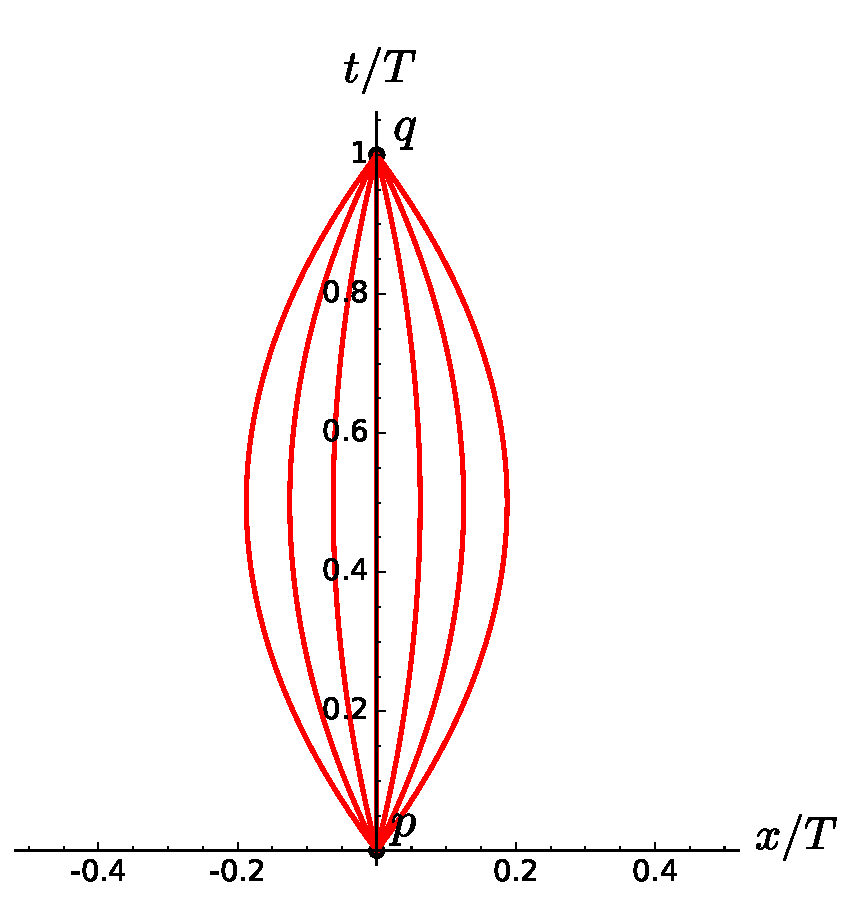
\includegraphics[height=0.3\textheight]{geo_timelike_h.pdf}}
\caption[]{\label{f:geo:timelike_h} \footnotesize
Timelike curves $\Li_h$ connecting the point $p$
of coordinates $(0,0,0,0)$ to the point $q$ of coordinates $(T,0,0,0)$
in Minkowski spacetime. From the left to right, the depicted curves
correspond to $h$ spanning $[-3/4, 3/4]$, with the step $\delta h = 1/4$.}
\end{figure}


\begin{example}[Timelike geodesic in Minkowski spacetime] \label{x:geo:timelike_geod_Mink}
Let us suppose that $(\M,\w{g})$ is the 4-dimensional Minkowski spacetime.
All geodesics are then (segments of) straight lines. If $p$ and $q$ are
connected by a timelike geodesic $\Li$,
we may consider a Minkowskian coordinate system $(x^\alpha)=(t,x,y,z)$
such that $x^\alpha(p) = (0,0,0,0)$ and $x^\alpha(q) = (T,0,0,0)$, for some $T>0$.
$t$ is then the proper time along $\Li$ and
$L_{(p,q)}(\Li)=T$. Let us consider the one-parameter family of curves
$(\Li_h)_{h\in(-1,1)}$ defined by $x^\alpha = X^\alpha(\lambda)$ with
$\lambda\in[0,T]$ and
\[
   X^0(\lambda) = \lambda, \quad
   X^1(\lambda) = \frac{h}{T} \lambda(T - \lambda),\quad
   X^2(\lambda) = 0, \quad
   X^3(\lambda) = 0 .
\]
Note that $X^0(\lambda) = \lambda$ means that the curve parameter
coincides with the time coordinate: $\lambda = t$.
We have $\Li_0 = \Li$ and for $h\not=0$, $\Li$ is
an arc of parabola from $p$ to $q$ in the $(t,x)$ plane
(cf. Fig.~\ref{f:geo:timelike_h}); the dimensionless
parameter $h$ is related to the curve's maximal extension along $x$ by
$x_{\rm max} = h T /4$. We have
\[
   \dot{X}^0(\lambda) = 1, \quad
   \dot{X}^1(\lambda) = h \left( 1 - 2\frac{\lambda}{T} \right),\quad
   \dot{X}^2(\lambda) = 0, \quad
   \dot{X}^3(\lambda) = 0 .
\]
Given that $(g_{\alpha\beta}) = \mathrm{diag}(-1,1,1,1)$, it follows that
$g_{\mu\nu} \dot{X}^\mu \dot{X}^\nu = -1 + h^2(1-2\lambda/T)^2$.
Since $\lambda\in[0,T]$, this shows that $\Li_h$ is a timelike
curve as long as $-1\leq h \leq 1$. Its length is
\[
L_{(p,q)}(\Li_h) = \int_{0}^{T} \sqrt{ 1 - h^2 \left( 1 - 2\frac{\lambda}{T} \right)^2 }
    \, \D\lambda  = \frac{T}{2h} \int_{-h}^h \sqrt{1 - u^2} \, \D u
    = \frac{T}{2h} \int_{-\mathrm{arcsin}\, h}^{\mathrm{arcsin}\, h}
        \cos^2 \theta \, \D \theta .
\]
Evaluating the integral leads to
\[
    L_{(p,q)}(\Li_h) = \frac{T}{2} \left( \sqrt{1-h^2} + \frac{\mathrm{arcsin}\, h}{h} \right) .
\]
Note that $\mathrm{arcsin}\, h/h$ is well defined at $h=0$, since
$\lim_{h\rightarrow 0}  \mathrm{arcsin}\, h/h = 1$.
The graph of $L_{(p,q)}(\Li_h)$ as a function $h$ is plotted in
Fig.~\ref{f:geo:timelike_length_h}. We see clearly that $h=0$, i.e. the
geodesic $\Li$, corresponds to the maximal length.
\end{example}

\begin{figure}
\centerline{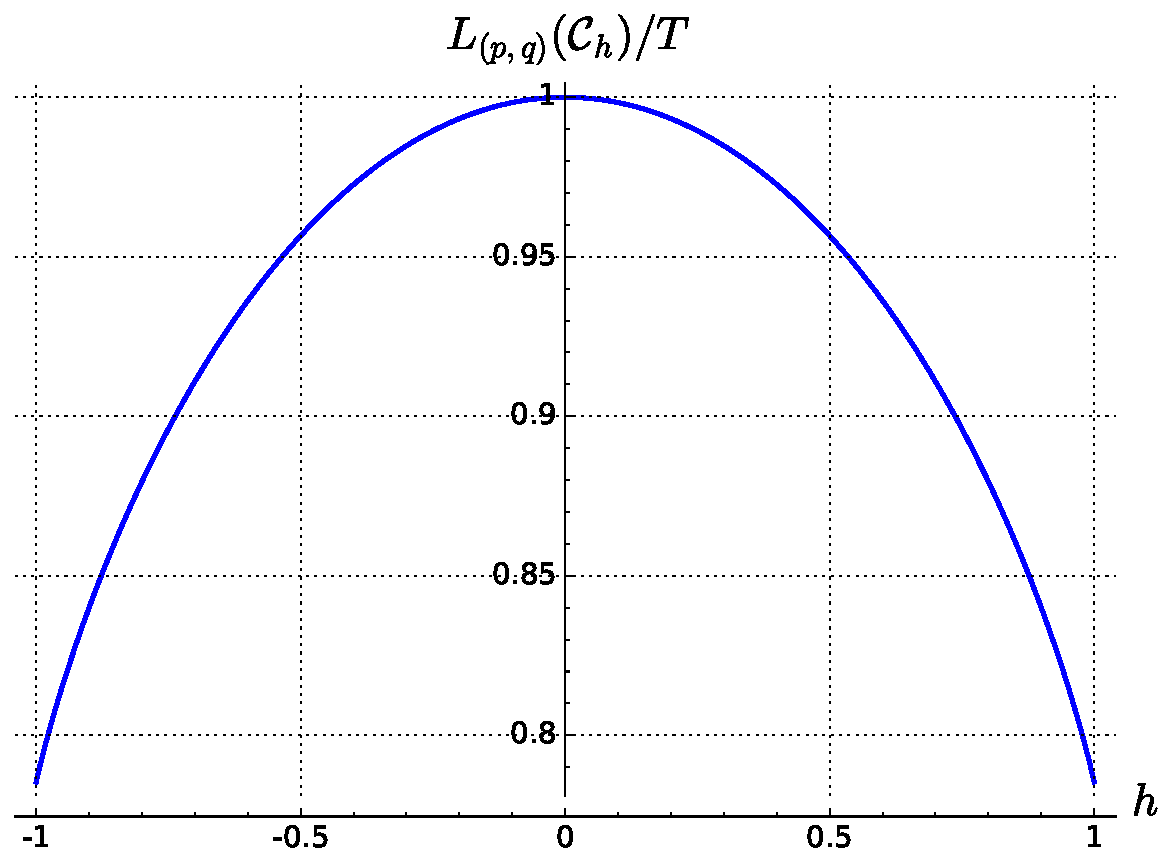
\includegraphics[height=0.3\textheight]{geo_timelike_length_h.pdf}}
\caption[]{\label{f:geo:timelike_length_h} \footnotesize
Length of the timelike curve $\Li_h$ connecting the point $p$
of coordinates $(0,0,0,0)$ to the point $q$ of coordinates $(T,0,0,0)$
in Minkowski spacetime, as a function of the parameter $h$ measuring
the deviation from the timelike geodesic $\Li=\Li_0$.}
\end{figure}


For a spacelike geodesic in a Lorentzian manifold,
the stationary length corresponds neither to a
maximum nor a minimum, but rather to a \emph{saddle point}, as the example
below illustrates.


\begin{example}[Spacelike geodesic in Minkowski spacetime]
As in Example~\ref{x:geo:timelike_geod_Mink}, we consider Minkowski spacetime,
but this time, $\Li$ is assumed to be a spacelike geodesic from $p$ to $q$. Since $\Li$ is necessarily a straight line
segment, without any loss of generality, we may introduce a Minkowskian coordinate
system $(x^\alpha)=(t,x,y,z)$ such that $x^\alpha(p) = (0,0,0,0)$ and
$x^\alpha(q) = (0,L,0,0)$ for some $L>0$, which is nothing but the length
$L_{(p,q)}(\Li)$ of the geodesic $\Li$. Any spacelike curve
$\Li'$ connecting $p$ and $q$ and lying in the hyperplane $\Sigma$
defined by $t=0$ obeys $L_{(p,q)}(\Li') \geq L_{(p,q)}(\Li)$
since $\Sigma$, equipped with the metric induced by $\w{g}$, is a
3-dimensional Euclidean space.

Let us consider some one-parameter family of curves
$(\Li_h)_{h\in(-1,1)}$ lying in the orthogonal complement of $\Sigma$
through $p$ and $q$, namely the curves defined $x^\alpha = X^\alpha(\lambda)$ with
$\lambda\in[0,L]$ and
\[
   X^0(\lambda) = \frac{h}{L} \lambda(L - \lambda), \quad
   X^1(\lambda) = \lambda, \quad
   X^2(\lambda) = 0, \quad
   X^3(\lambda) = 0 .
\]
As in Example~\ref{x:geo:timelike_geod_Mink}, we have $\Li_0=\Li$
and for $h\not=0$, the $\Li_h$'s are
arcs of parabola from $p$ to $q$, which remain spacelike as long as
$-1<h<1$ (cf. Fig.~\ref{f:geo:spacelike_h}).
The computations are similar to those of Example~\ref{x:geo:timelike_geod_Mink},
leading to
\[
    L_{(p,q)}(\Li_h) = \frac{L}{2} \left( \sqrt{1-h^2} + \frac{\mathrm{arcsin}\, h}{h} \right) .
\]
$L_{(p,q)}(\Li_h) / L$ is exactly the same of function of $h$
as $L_{(p,q)}(\Li_h) / T$ in Example~\ref{x:geo:timelike_geod_Mink}.
In view of Fig.~\ref{f:geo:timelike_length_h}, we therefore assert
that $L_{(p,q)}(\Li_h) \leq L_{(p,q)}(\Li)$.

We conclude that the spacelike geodesic $\Li$ corresponds to a
saddle point of the length functional: it is a minimum among the curves lying
in the $(x,y,z)$ hyperplane but a maximum among those lying in the $(t,x)$
plane.
\end{example}

\begin{figure}
\centerline{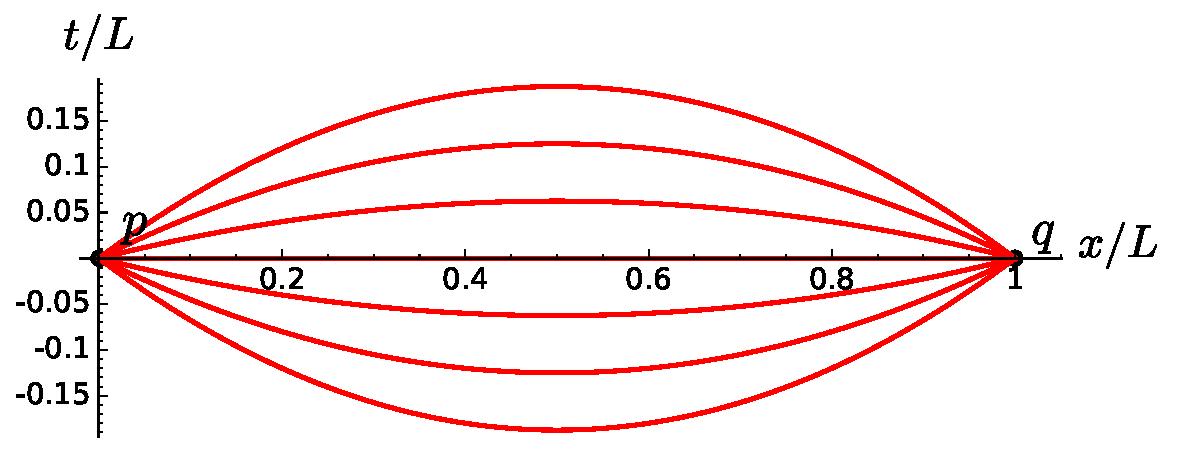
\includegraphics[width=0.7\textwidth]{geo_spacelike_h.pdf}}
\caption[]{\label{f:geo:spacelike_h} \footnotesize
Spacelike curves $\Li_h$ connecting the point $p$
of coordinates $(0,0,0,0)$ to the point $q$ of coordinates $(0,L,0,0)$
in Minkowski spacetime. From the bottom to the top, the depicted curves
correspond to $h$ spanning $[-3/4, 3/4]$, with the step $\delta h = 1/4$.}
\end{figure}


\subsection{All geodesics as stationary points of some action} \label{s:geo:all_geod}

We have excluded null geodesics from the above variational analysis by
invoking the necessary smoothness of the Lagrangian (\ref{e:geo:Lagrangian}).
We may further convince ourselves that null geodesics would not have fit
in the analysis by noticing the division by $\mathcal{L}$ in Eq.~(\ref{e:geo:kappa_from_L}),
which excludes $\mathcal{L} = 0$.
However, it is possible to get all geodesics, including the null ones, from
a variational principle; one has to start from a different action, namely
\be \label{e:geo:energy_funct}
    S_{(p,q)}(P) := \frac{1}{2}\int_{\lambda_p}^{\lambda_q}
        g_{\mu\nu}(X^\rho) \dot{X}^\mu \dot{X}^\nu \, \D\lambda ,
\ee
where $P$ is a parametrization of the curve $\Li$, $\lambda$
the corresponding parameter
and $x^\alpha = X^\alpha(\lambda)$ the coordinate expression of $P$.

The Lagrangian in (\ref{e:geo:energy_funct}) is
\be \label{e:geo:Lagrangian2}
   \mathcal{L}_2(X^\alpha, \dot{X}^\alpha) =  \frac{1}{2}
        g_{\mu\nu}(X^\rho) \dot{X}^\mu \dot{X}^\nu  .
\ee
We notice that it is always differentiable, even
when $g_{\mu\nu}\dot{X}^\mu \dot{X}^\nu  = 0$, i.e. it allows for null curves.
However the price to pay is that,
contrary to the length (\ref{e:geo:def_length_X}),
the action depends on the parametrization of the curve,
hence the notation $S_{(p,q)}(P)$ rather than $S_{(p,q)}(\Li)$.
For this reason, $S_{(p,q)}(P)$ is not expected to have any significant
physical meaning, contrary to $L_{(p,q)}(\Li)$, which is the proper
time along timelike curves.

Searching for stationary points of the action
(\ref{e:geo:energy_funct}) is straightforward. Indeed,
given Eqs.~(\ref{e:geo:der_gXX_X}) and (\ref{e:geo:der_gXX_X_dot}),
we have
\[
    \der{\mathcal{L}_2}{X^\alpha} = \frac{1}{2}
        \der{g_{\mu\nu}}{x^\alpha}  \dot{X}^\mu \dot{X}^\nu
    \qquad\mbox{and}\qquad
    \der{\mathcal{L}_2}{\dot{X}^\alpha} = g_{\alpha\mu} \dot{X}^\mu ,
\]
so that
\[
    \frac{\D}{\D\lambda}\left( \der{\mathcal{L}_2}{\dot{X}^\alpha}\right) =
      \der{g_{\alpha\mu}}{x^\nu} \dot{X}^\nu \dot{X}^\mu
      + g_{\alpha\mu} \ddot{X}^\mu .
\]
Using the identity (\ref{e:geo:gXX_indices}), the Euler-Lagrange equation
(\ref{e:geo:Euler-Lagrange}) (with $\mathcal{L}$ substituted by $\mathcal{L}_2$)
turns out to be equivalent to the geodesic equation (\ref{e:geo:eq_geod}).
We conclude that
\begin{greybox}
In a pseudo-Riemannian manifold $(\M,\w{g})$, a
curve $\Li$ equipped with a parametrization $P$
is a stationary point of the action (\ref{e:geo:energy_funct})
iff $\Li$ is a geodesic and $P$ an affine parametrization of it.
\end{greybox}

\begin{remark}
The variational principle applied to the action (\ref{e:geo:energy_funct}) leads directly
to the geodesic equation (\ref{e:geo:eq_geod}), which implies that the
involved parametrization is affine. On the contrary,
the variation of the length functional (\ref{e:geo:def_length_X}),
leads only to the pregeodesic equation
(\ref{e:geo:pregeod_eq_comp}) (cf. the computation in Sec.~\ref{s:geo:variation_length}),
which permits a generic parametrization of the geodesic, in agreement with
the fact that the length is parametrization-independent, contrary to the
action (\ref{e:geo:energy_funct}).
\end{remark}

\begin{remark}
The factor $1/2$ in Eq.~(\ref{e:geo:energy_funct}) does not play any role
in the variational principle, so we could have dropped it. However, thanks to
it, the momentum conjuguate to $X^\alpha$ takes a simple form:
\be
    \Pi_\alpha := \der{\mathcal{L}}{\dot{X}^\alpha} = g_{\alpha\mu} \dot{X}^\mu .
\ee
The Lagrangian (\ref{e:geo:Lagrangian2}) can be then written
$\mathcal{L}_2 = 1/2\, \Pi_\mu \dot{X}^\mu$ and the
Hamiltonian\index{Hamiltonian!for geodesic motion}
deduced from it by the standard Legendre transformation is
$\mathcal{H} = \Pi_\mu \dot{X}^\mu - \mathcal{L}_2 = 1/2\, \Pi_\mu \dot{X}^\mu$,
i.e.
\be
    \mathcal{H}(X^\alpha, \Pi_\alpha) = \frac{1}{2} g^{\mu\nu}(X^\rho) \Pi_\mu \Pi_\nu .
\ee
Such a Hamiltonian has been used by Carter \cite{Carte68}
to study the geodesics in Kerr spacetime,
discovering the famous \emph{Carter constant}\index{Carter constant}.
\end{remark}

%%%%%%%%%%%%%%%%%%%%%%%%%%%%%%%%%%%%%%%%%%%%%%%%%%%%%%%%%%%%%%%%%%%%%%%%%%%%%%%


\section{Geodesics and symmetries} \label{s:geo:sym}

\subsection{Killing vector}

As a reminiscence of Noether's theorem\index{Noether's theorem},
symmetries in a pseudo-Riemannian manifold lead to conserved
quantities along geodesics.
Let us first recall that 1-dimensional
groups of symmetry and the related concept of Killing vector field
have been introduced in Sec.~\ref{s:neh:symmetries}. In terms of them,
we may state the following conservation law:

\begin{greybox}
If the pseudo-Riemannian manifold $(\M,\w{g})$ admits a 1-dimensional
group of symmetry of generator $\w{\xi}$, i.e. $\w{\xi}$ is a Killing
vector field of $(\M,\w{g})$, then along any geodesic $\Li$,
the $\w{g}$-scalar product of $\w{\xi}$ by any tangent vector field
$\w{v}=\D\w{x}/\D\lambda$ associated with an
affine parameter $\lambda$ of $\Li$ is constant:
\be
    \w{g}(\w{\xi},\w{v}) = \mathrm{const} .
\ee
\end{greybox}

\begin{proof}
The variation of $\w{g}(\w{\xi},\w{v})$ along $\Li$ is,
according to Eq.~(\ref{e:bas:def_vector}),
\bea
    \frac{\D}{\D\lambda} \, \w{g}(\w{\xi},\w{v}) & = & \w{v}\left( \w{g}(\w{\xi},\w{v}) \right) =
        \wnab_{\!\w{v}} \left( \w{g}(\w{\xi},\w{v}) \right) \nonumber \\
        & = & v^\sigma \nabla_\sigma ( g_{\mu\nu} \xi^\mu v^\nu ) =
        v^\sigma \nabla_\sigma (\xi_\nu v^\nu ) = \nabla_\sigma \xi_\nu \, v^\sigma  v^\nu
            + \xi_\nu v^\sigma \nabla_\sigma v^\nu \nonumber \\
        & = & \frac{1}{2} (\underbrace{\nabla_\sigma \xi_\nu + \nabla_\mu \xi_\sigma}_{0}) v^\sigma  v^\nu
            +  \xi_\nu \underbrace{v^\sigma \nabla_\sigma v^\nu}_{0}  = 0, \label{e:geo:dem_conservation}
\eea
where the first zero holds because $\w{\xi}$ obeys to the Killing equation
(\ref{e:neh:Killing_equation}) and the second one holds thanks to
Eq.~(\ref{e:geo:geod_eq_v}), which expresses that $\Li$ is a geodesic
and $\w{v}$ the tangent vector associated with some affine parameter.
\end{proof}

\begin{remark}
If the tangent vector $\w{v}$ is associated with a generic (not necessarily affine)
parameter of $\Li$, the second zero in Eq.~(\ref{e:geo:dem_conservation})
must be replaced by $\kappa v^\nu$, where $\kappa$ is the non-affinity
coefficient of $\w{v}$ [cf. Eq.~(\ref{e:geo:v_pregeodesic})]. Accordingly
$\w{g}(\w{\xi},\w{v})$ is no longer constant along $\Li$ but rather
evolves according to
\be
    \frac{\D}{\D\lambda} \, \w{g}(\w{\xi},\w{v}) = \kappa \, \w{g}(\w{\xi},\w{v}) .
\ee
Note that $\kappa$ a priori varies along $\Li$, so that the integration of
this first-order differential equation depends of the precise form of the
function $\kappa(\lambda)$.
\end{remark}

\subsection{Killing tensor}

\begin{greybox}
A \defin{Killing tensor}\index{Killing!tensor} of rank $p\geq 1$ in the
pseudo-Riemannian manifold $(\M,\w{g})$ is a tensor field $\w{K}$ of type $(0,p)$
that is fully symmetric and whose covariant derivative is fully antisymmetric:
\be
    \nabla_{(\alpha_1} K_{\alpha_2\ldots\alpha_{p+1})} = 0 .
\ee
\end{greybox}

\begin{example}
A trivial example is the metric tensor $\w{g}$ itself.
If $(\M,\w{g})$ admits a Killing vector $\w{\xi}$, other examples
are for $p=1$: $\w{K} = \uu{\xi}$ (by Killing equation (\ref{e:neh:Killing_equation})),
for $p=2$:
$\w{K} = \uu{\xi} \otimes \uu{\xi}$ (by the Leibnitz rule + the Killing equation),
for $p=3$: $\w{K} = \uu{\xi} \otimes \uu{\xi} \otimes \uu{\xi}$ (idem), etc.
\end{example}

\begin{greybox}
If $\w{K}$ is a Killing tensor of rank $p$ on the
the pseudo-Riemannian manifold $(\M,\w{g})$, then along any geodesic $\Li$,
the scalar $\w{K}(\w{v},\ldots,\w{v})$, where $\w{v}=\D\w{x}/\D\lambda$ is any tangent vector field associated with an
affine parameter $\lambda$ of $\Li$, is constant:
\be \label{e:geo:Kvv_const}
    \w{K}(\w{v},\ldots,\w{v}) = \mathrm{const} .
\ee
\end{greybox}

\begin{example}
Since we have already noticed that the metric tensor $\w{g}$ is a Killing tensor,
the property (\ref{e:geo:vv_const}) appears as a special case of (\ref{e:geo:Kvv_const}).
\end{example}

